\documentclass[runningheads,a4paper]{llncs}
\usepackage{amssymb}
\usepackage{tikz}
\usetikzlibrary{automata,positioning,arrows,shapes,fit}
\usepackage{pgfplots}
\pgfplotsset{width=10cm,compat=1.9}

\begin{document}

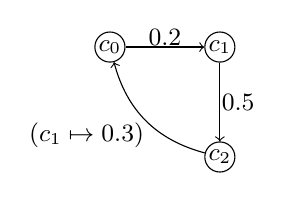
\begin{tikzpicture}[initial text={},inner sep=0.5pt,minimum size=0mm,every
  node/.style={font=\small},every state/.style={minimum size=0mm}]
    \node[state](c0){$c_0$};
    \node[state,right= of c0](c1){$c_1$};
    \node[state,below= of c1](c2){$c_2$};

    \path[->,auto]
    (c0) edge node[above]{$0.2$} (c1)
    (c1) edge node{$0.5$} (c2)
    (c2) edge[bend left] node{$(c_1 \mapsto 0.3)$} (c0);
\end{tikzpicture}

\end{document}